% !TeX encoding = UTF-8
% !TeX spellcheck = en_US
% !TeX root = ../../Thesis.tex

\chapter{Beam Characterization}
\label{ch:Beam Characterization}

Chapter about beam characterization.

\noindent \textcolor{red}{ignore from here} \\
2019-09-27 set voltages \\
2019-09-30 first successful external run \\
2019-10-07 spot vs pressure \\
2019-10-22 wobble stick measurement \\
2019-11-05 forgot to turn off filament heating \\
2019-11-14 assemble chamber with copper rings \\
2019-11-18 Faraday cup measurement, and next day variation \\
\textcolor{red}{to here}

\noindent \textbf{possible sections} \\
current and voltage on filament \\
pressure (oxygen exposure) vs beam current \\
aluminum foil \\
What happens with the wobblestick ->  \\
Faraday cup -> Frank \\
Beam current measurement -> Frank \\
Measurement Ablenkungsgeschwindigkeit (frequency) -> Alex \\


\section{Aluminum foil}
\label{sec:Aluminum foil}

In \cref{fig:Front view of vacuum chamber (first iteration)} the inside of the 6-way cross of the first iteration is shown. On one side of the phosphor screen, aluminum foil was attached to simulate the aquadag coating inside a CRT\todo{explain in basics what aquadag is?}. The beam was deflected on the aluminum foil and the BNC output was connected to ground through an ammeter to measure the beam current. As shown in \cref{fig:Difference in filament voltage and beam current between an opened and unopened CRT} there is close to no difference in the filament voltage (and therefore heating power) between an opened and unopened CRT while the beam current on the aluminum foil varies widely. One possible reason could be that electrons scatter around and not all choose the wire path to ground. Therefore a Faraday cup (see \todo{ref Faraday cup section}) was used in the second iteration.


\begin{figure}[h]
	\centering
	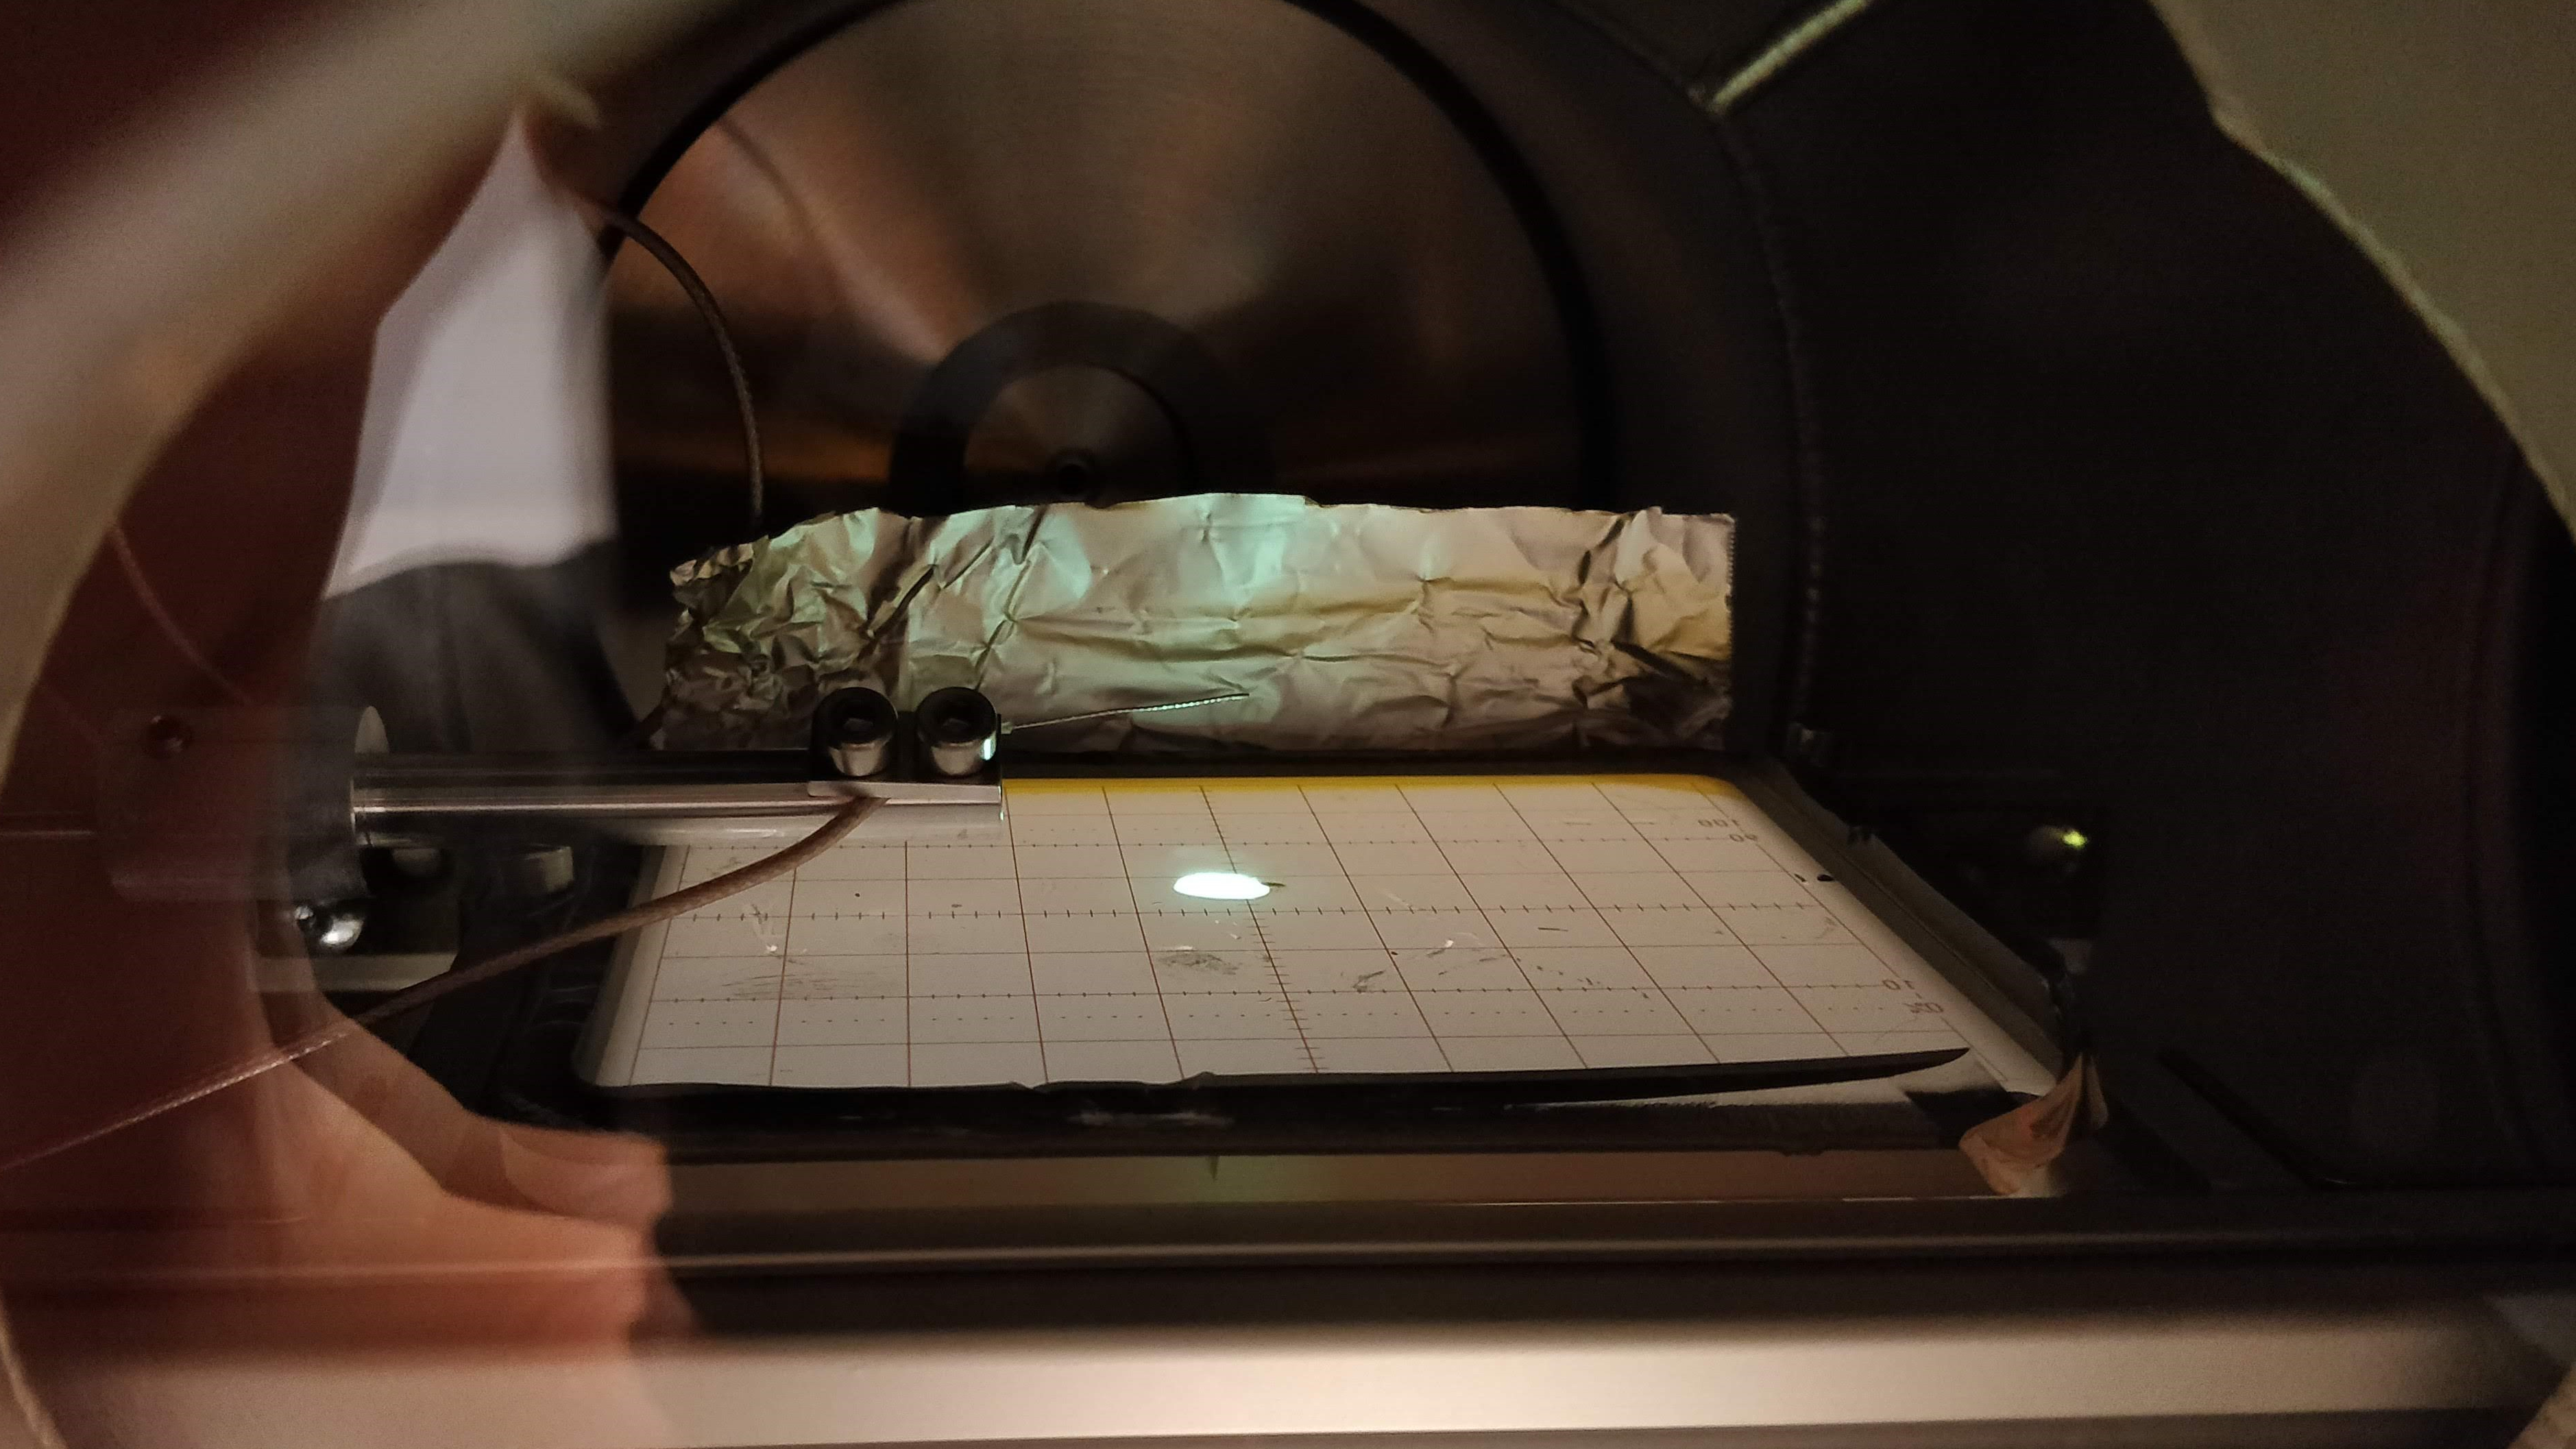
\includegraphics[width=0.9\textwidth]{./Chapters/beam-characterization/center_image}
	\caption{Front view of vacuum chamber (first iteration).}
	\label{fig:Front view of vacuum chamber (first iteration)}
\end{figure}


\begin{figure}[ht]
	\centering
	
	\begin{tikzpicture}
		% !TeX encoding = UTF-8
% !TeX spellcheck = en_US
% !TeX root = ../../Thesis.tex

\begin{groupplot}[
		group style={
			group size=2 by 1,
			horizontal sep=0.15\textwidth}, %0.1\textwidth},
		width=0.5\textwidth,
		height=0.5\textwidth]
	
	%1st plot
	\nextgroupplot[
		%title={},
		xlabel={filament current/\si{\milli\ampere}},
		ylabel={filament voltage/\si{\volt}},
	%	xmin=5, xmax=7.5,
	%	ymin=0, ymax=0.5,
		legend style={at={(0.05, 0.95)}, anchor={north west}},
		legend cell align={left}]
	
	\addplot+[
		black,
		only marks,
		mark=*,
		mark size=2pt,
		mark options={solid}]
	table [x=current_filament, y=voltage, col sep=comma]{./Chapters/beam-characterization/data_aluminum_foil_opened.csv};
	\addlegendentry{open}
	
	\addplot+[
		blue,
		only marks,
		mark=*,
		mark size=2pt,
		mark options={solid}]
	table [x=current_filament, y=voltage, col sep=comma]{./Chapters/beam-characterization/data_aluminum_foil_sealed.csv};
	\addlegendentry{sealed}
	

%	%2nd plot
	\nextgroupplot
	[
	%title={},
	xlabel={filament current/\si{\milli\ampere}},
	ylabel={beam current/\si{\micro\ampere}},
%	xmin=5, xmax=7.5,
	ymin=0, %ymax=0.5,
	legend style={at={(0.05, 0.95)}, anchor={north west}},
	legend cell align={left},
	]
	
	\addplot+[
		black,
		only marks,
		mark=*,
		mark size=2pt,
		mark options={solid}	]
	table [x=current_filament, y=current, col sep=comma]{./Chapters/beam-characterization/data_aluminum_foil_opened.csv};
	\addlegendentry{open}
	
	\addplot+[
		blue,
		only marks,
		mark=*,
		mark size=2pt,
		mark options={solid}]
	table [x=current_filament, y=current, col sep=comma]{./Chapters/beam-characterization/data_aluminum_foil_sealed.csv};
	\addlegendentry{sealed}
\end{groupplot}
	\end{tikzpicture}
	
	\caption{Difference in filament voltage and beam current between an opened and unopened CRT.}
	\label{fig:Difference in filament voltage and beam current between an opened and unopened CRT}
	\todo[inline]{figure size, overfull hbox}
\end{figure}

\section{Faraday cup}\todo[caption{error with figures}]{Package tikz Error: Sorry, the system call 'pdflatex -halt-on-error -interact}
\label{sec:Faraday cup}


In order to accurately measure the beam current, a Faraday cup was built. A schematic is shown in \cref{fig:Schematics of Faraday cup}. A copper tube was cut at an \ang{45} angle on one side and a Cu-sheet was soldered at the top and bottom. A small hole \todo{diameter?} was drilled at the top and a coaxial cable was attached on the mantle which connects to a BNC feedthrough at the top of the chamber. The small opening and bent floor were made in order to reduce backscattering as indicated by blue arrows. At the top surface a phosphor coating was applied in order to make the beam visible which made it easier to guide it into the opening hole.


%\begin{figure}[h]
%	\centering
%	\begin{tikzpicture}
%		% !TeX encoding = UTF-8
% !TeX spellcheck = en_US
% !TeX root = ../../Thesis.tex


%\draw [help lines] (-2, -2) grid (2, 5);


% cup
\draw (-0.3, 4) -- (-1, 4) -- (-1, -1) -- (1, 1) -- (1, 4) -- (0.3, 4);

% electron beam
\draw [blue] (0, 5) -- (0, 0);
\draw [blue, ->] (0, 0) -- (-1, -0.5);
\draw [blue, ->] (0, 0) -- (-1, 0.5);
\draw [blue, ->] (0, 0) -- (-1, 2);
\draw [blue, ->] (0, 0) -- (1, 2);
\node [right] at (1, 5) {\textcolor{blue}{e-beam}};

% 45 degree angle
\draw [dashed] (-1, -1) -- (2, -1);
\draw(-1+2, -1)arc [start angle=0,end angle=45, radius=2];
\node [right] at (1, 0) {\ang{45}};

% phosphor coating
\draw [fill=green] (-1, 4) rectangle (-0.3 , 4.1);
\draw [fill=green] (0.3, 4) rectangle (1, 4.1);
\node [right] at (1, 4.05) {\textcolor{green}{phosphor coating}};
%	\end{tikzpicture}
%	
%	\caption{Schematics of Faraday cup.}
%	\label{fig:Schematics of Faraday cup}
%\end{figure}

With this improved setup, the beam current was measured again. A summary is shown in \cref{fig:Beam current dependence on heater current}. It can be seen that a current of over \SI{300}{\micro\ampere} was achieved, which is more than the necessary amount for the experiment. A problem is the fact, that the current is not stable. A measurement on the next day under the same settings resulted in a current between \SIrange{50}{120}{\micro\ampere}.


%\begin{figure}[h]
%	\centering
%	\begin{tikzpicture}
%		% !TeX encoding = UTF-8
% !TeX spellcheck = en_US
% !TeX root = ../../Thesis.tex


	
%	%1st plot
%	\nextgroupplot[
%		%title={},
%		xlabel={filament current/\si{\milli\ampere}},
%		ylabel={filament voltage/\si{\volt}},
%	%	xmin=5, xmax=7.5,
%	%	ymin=0, ymax=0.5,
%		legend style={at={(0.05, 0.95)}, anchor={north west}},
%		legend cell align={left}]


\begin{axis}[
		%title={},
		xlabel={filament current/\si{\milli\ampere}},
		ylabel={beam current/\si{\micro\ampere}},
		%xmin=5, xmax=7.5,
		%ymin=0, ymax=0.5,
		%legend style={at={(0.05, 0.95)}, anchor={north west}},
		%legend cell align={left}]
	]
	\addplot[
		black,
		only marks,
		mark=*,
		mark size=2pt,
		mark options={solid},
	]
	table [x=current_filament, y=current_beam, col sep=comma]{./Chapters/beam-characterization/data_Faraday_cup.csv};
\end{axis}
%	\end{tikzpicture}
%	
%	\caption{Beam current dependence on heater current.}
%	\label{fig:Beam current dependence on heater current}
%\end{figure}
